%%%%%%%%%%%%%%%%%%%%%%%%%%%%%%%%%%%%%%%%%%%%%%%%%%%%%%
%% Fleet dynamics models in FLBEIA
%%%%%%%%%%%%%%%%%%%%%%%%%%%%%%%%%%%%%%%%%%%%%%%%%%%%%%

\documentclass[12pt, halfline, a4paper]{ouparticle}

\usepackage[utf8]{inputenc}
\usepackage{lscape}
\usepackage{rotating}

%%%%%%%%%%%%%%%%%%%%%%%%%%%%%%%%%%%%
\begin{document}

\title{Working title: Fleet dynamics models in FLBEIA}

\author{
	\name{Paul J. Dolder}
	\address{GMIT}
	\email{paul.dolder@research.gmit.ie}
	\address{CEFAS}
	\email{paul.dolder@cefas.co.uk\thanks{Corresponding author} }
	\and
	\name{Cóilín Minto}
	\address{GMIT}
	\email{coilin.minto@gmit.ie}
	\and
	\name{Dorleta Garcia}
	\address{AZTI}
	\email{dgarcia@azti.es}
}

\abstract{Some text here}

\date{\today}

\keywords{MSE, mixed fisheries, fleet dynamics, RUM, Markov}

\maketitle

\section{Introduction}
\label{intro}

Most fisheries worldwide are mixed. Evaluation of management performance still
based on single-species, failing to take account of fleet dynamics; technical
(mixed-fishery) interactions affect the outcome of management measures,
therefore important for MSEs to take account of mixed fisheries interactions.
\\

Location choice key decision that effects catch in mixed fisheries.\\

FLBEIA extension to include commonly used fleet dynamics models.	\\


\section{Methods}
\label{meth}

\begin{itemize}
	\item Implement fleet dynamics models in FLBEIA
	\item Fit models
		\begin{itemize}
			\item Gravity
			\item Gravity + tradition
			\item Markov
			\item RUM
		\end{itemize}
	\item Condition seasonal FLBEIA model
		\begin{itemize}
			\item 4 seasons
			\item Metiers defined by spatial patterns in catch
			\item Implement fleet dynamics model for Irish otter
				trawlers
		\end{itemize}
	\item Simulations including closures
		\begin{itemize}
			\item Close a metier, how does effect reallocate
		\end{itemize}
	\item MSE with different fleet dynamics models as OM
\end{itemize}

\section{Results}
\label{res}

\section{Discussion}
\label{dis}

\section{Conclusions}
\label{con}


\begin{notes}[Acknowledgements]
The authors would like to thank...
\end{notes}

\begin{thebibliography}
ggg
\end{thebibliography}


\newpage

\begin{figure}[!ht]
	\centering
	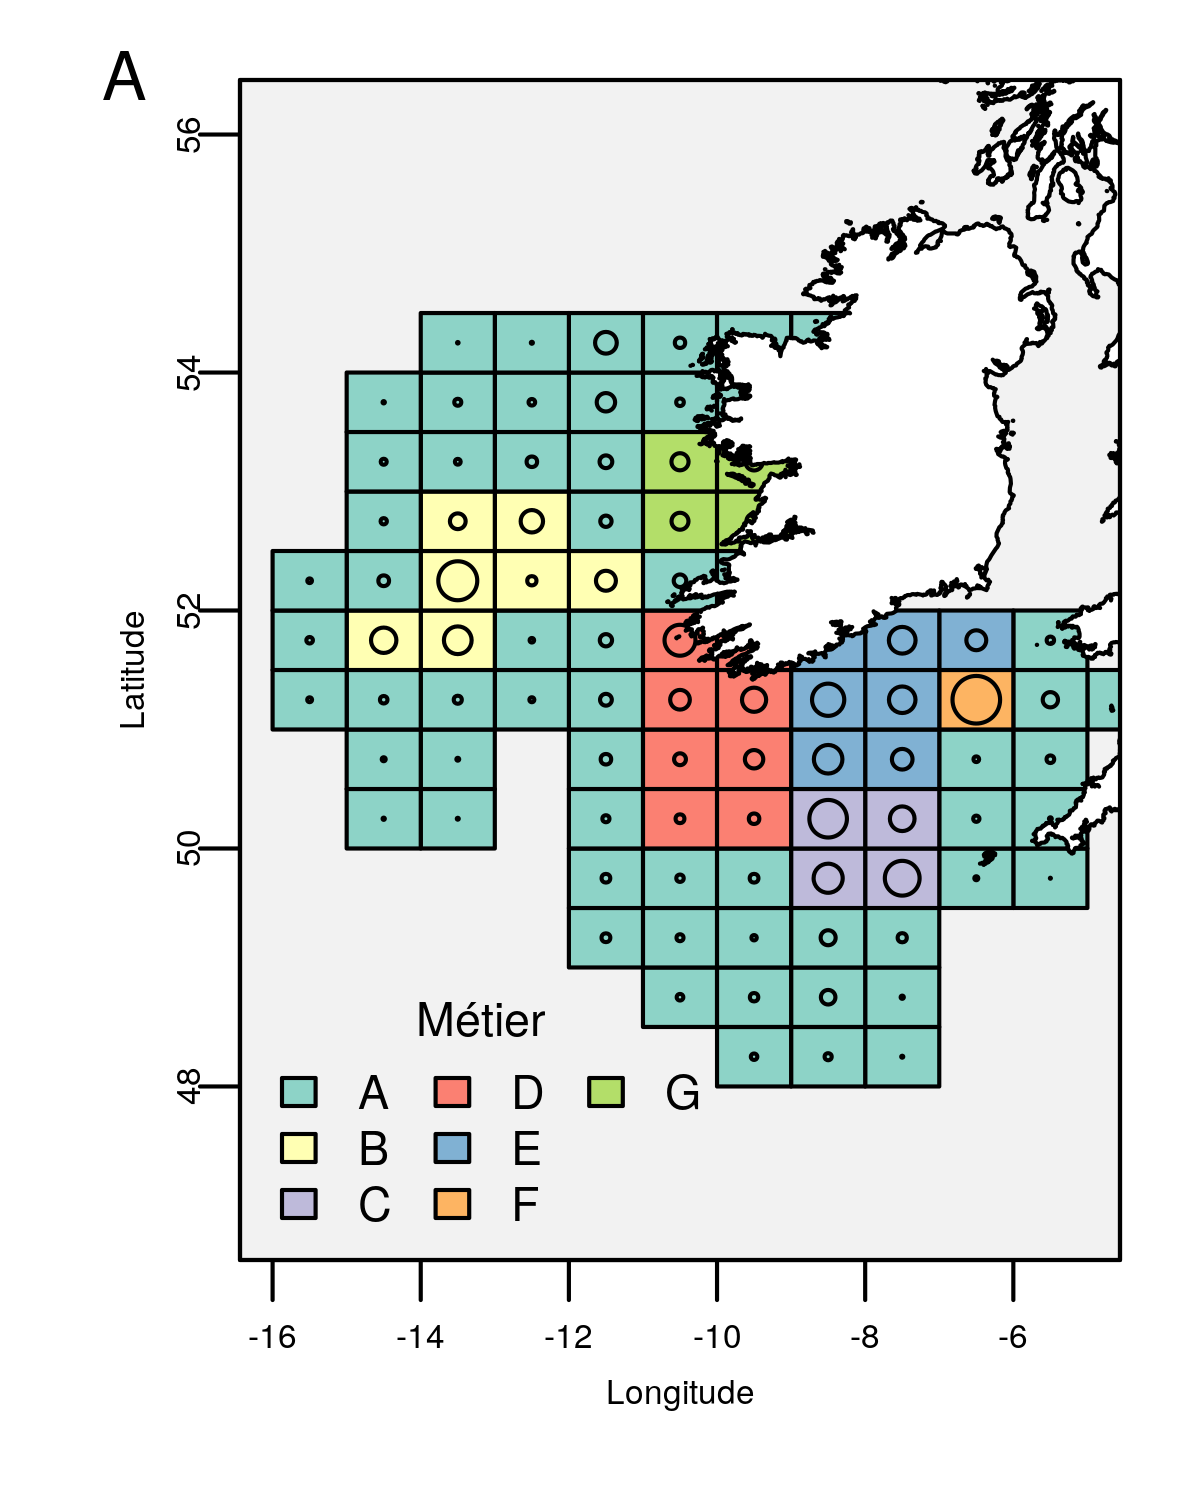
\includegraphics[width=0.8\linewidth]{figures/Final_Metier_locations}
	\caption{The defined spatial metier} 
	\label{fig:metier}
\end{figure}	

\begin{figure}[!ht]
	\centering
	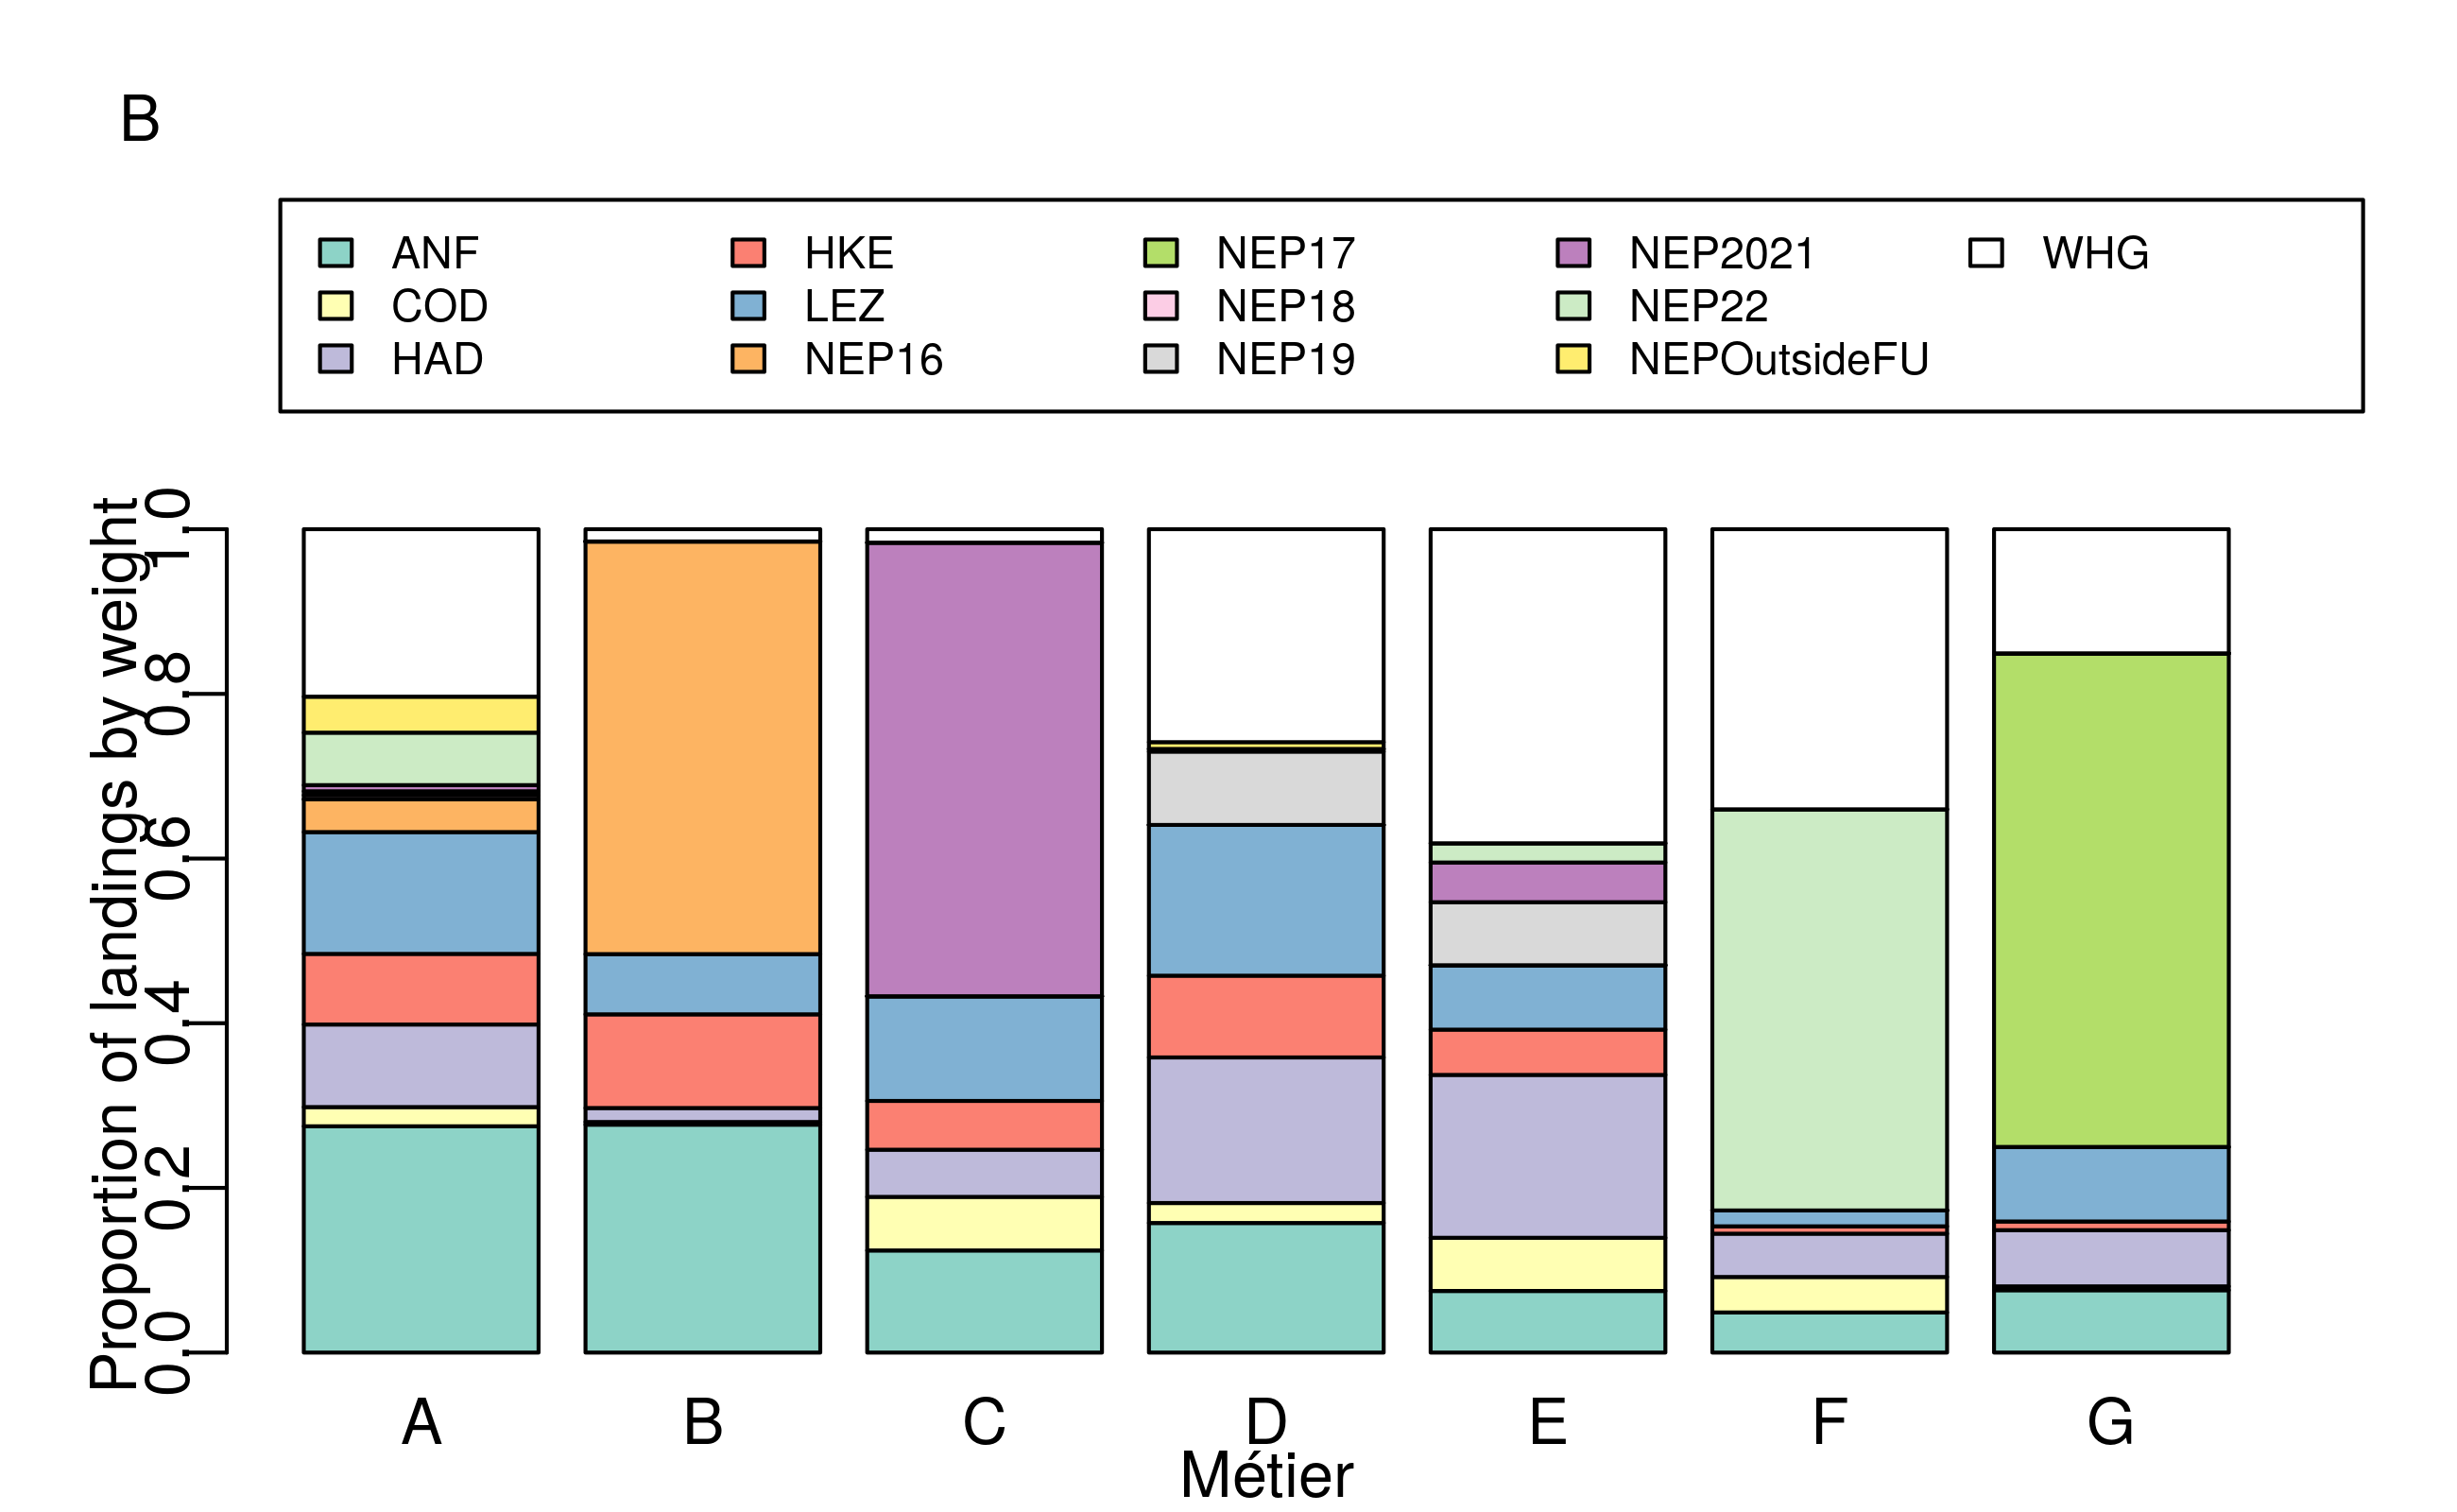
\includegraphics[width=0.8\linewidth]{figures/Final_Metier_catchcomp}
	\caption{Catch comp for metier} 
	\label{fig:catchcomp}
\end{figure}	

\newpage

\begin{sidewaysfigure}[!ht]
	\centering
	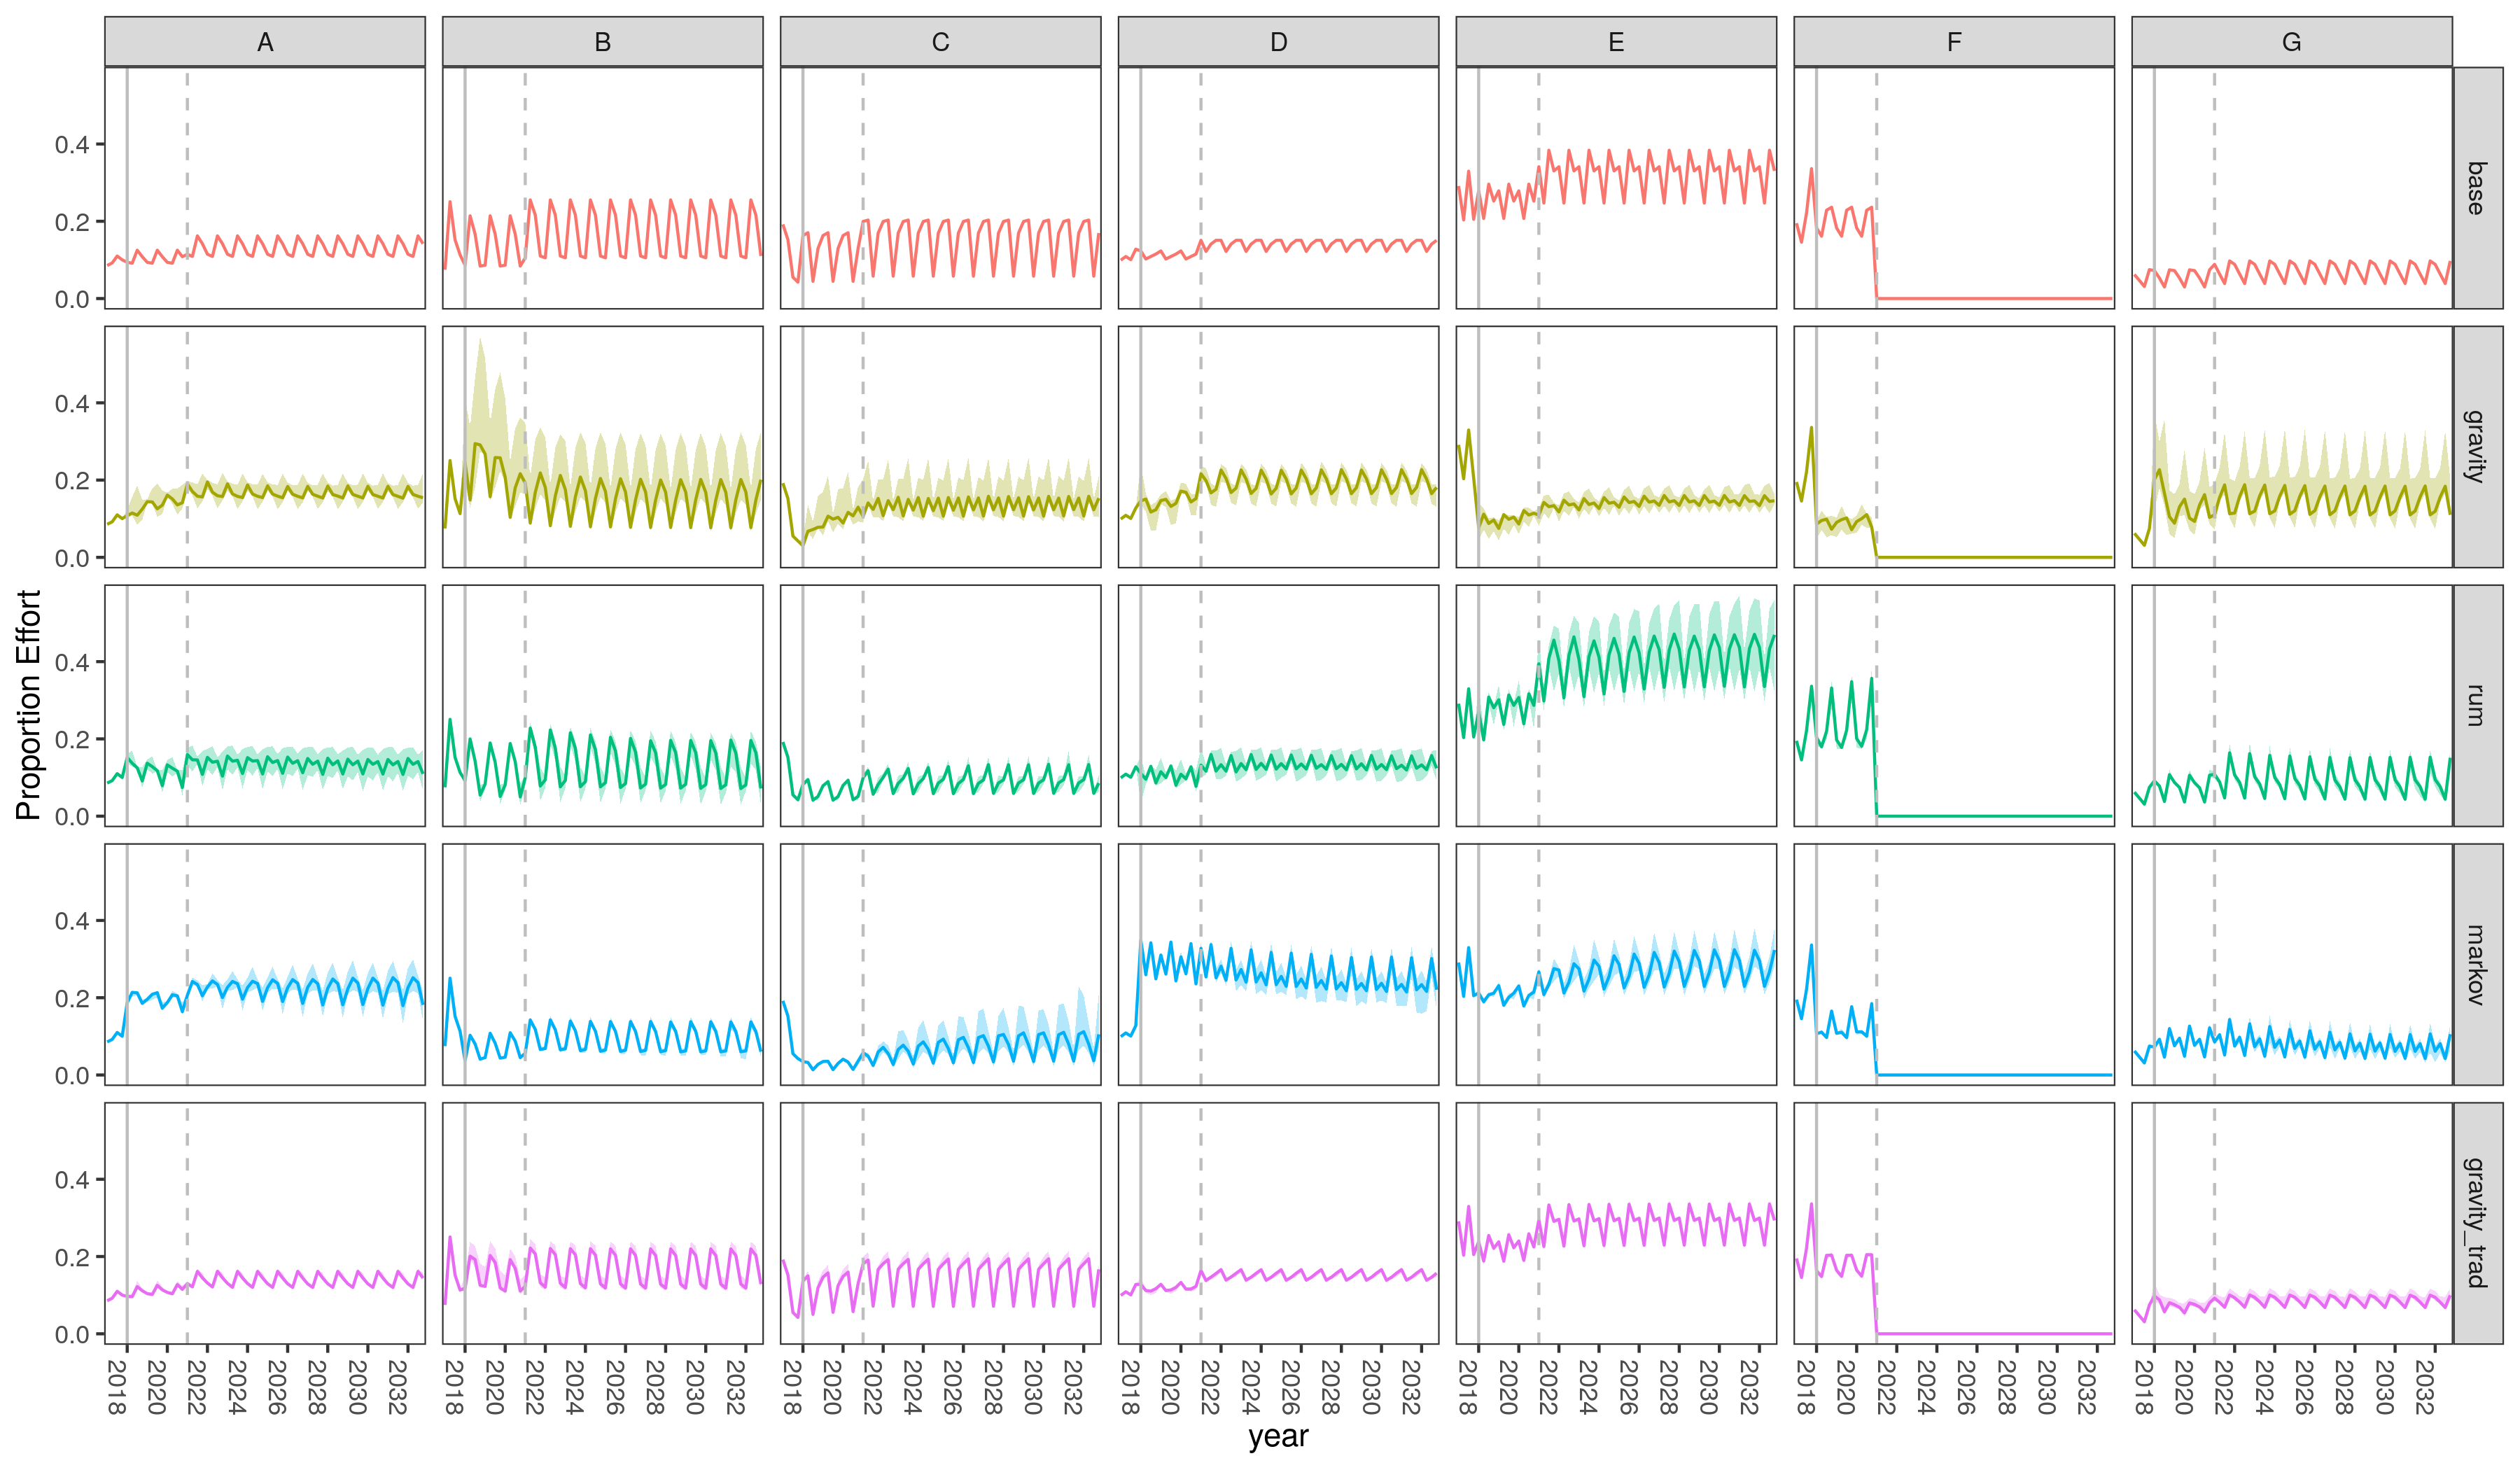
\includegraphics[width=1\linewidth]{figures/Effort_shares}
	\caption{Effort per location model} 
	\label{fig:effort}
\end{sidewaysfigure}	

\newpage

\begin{figure}[!ht]
	\centering
	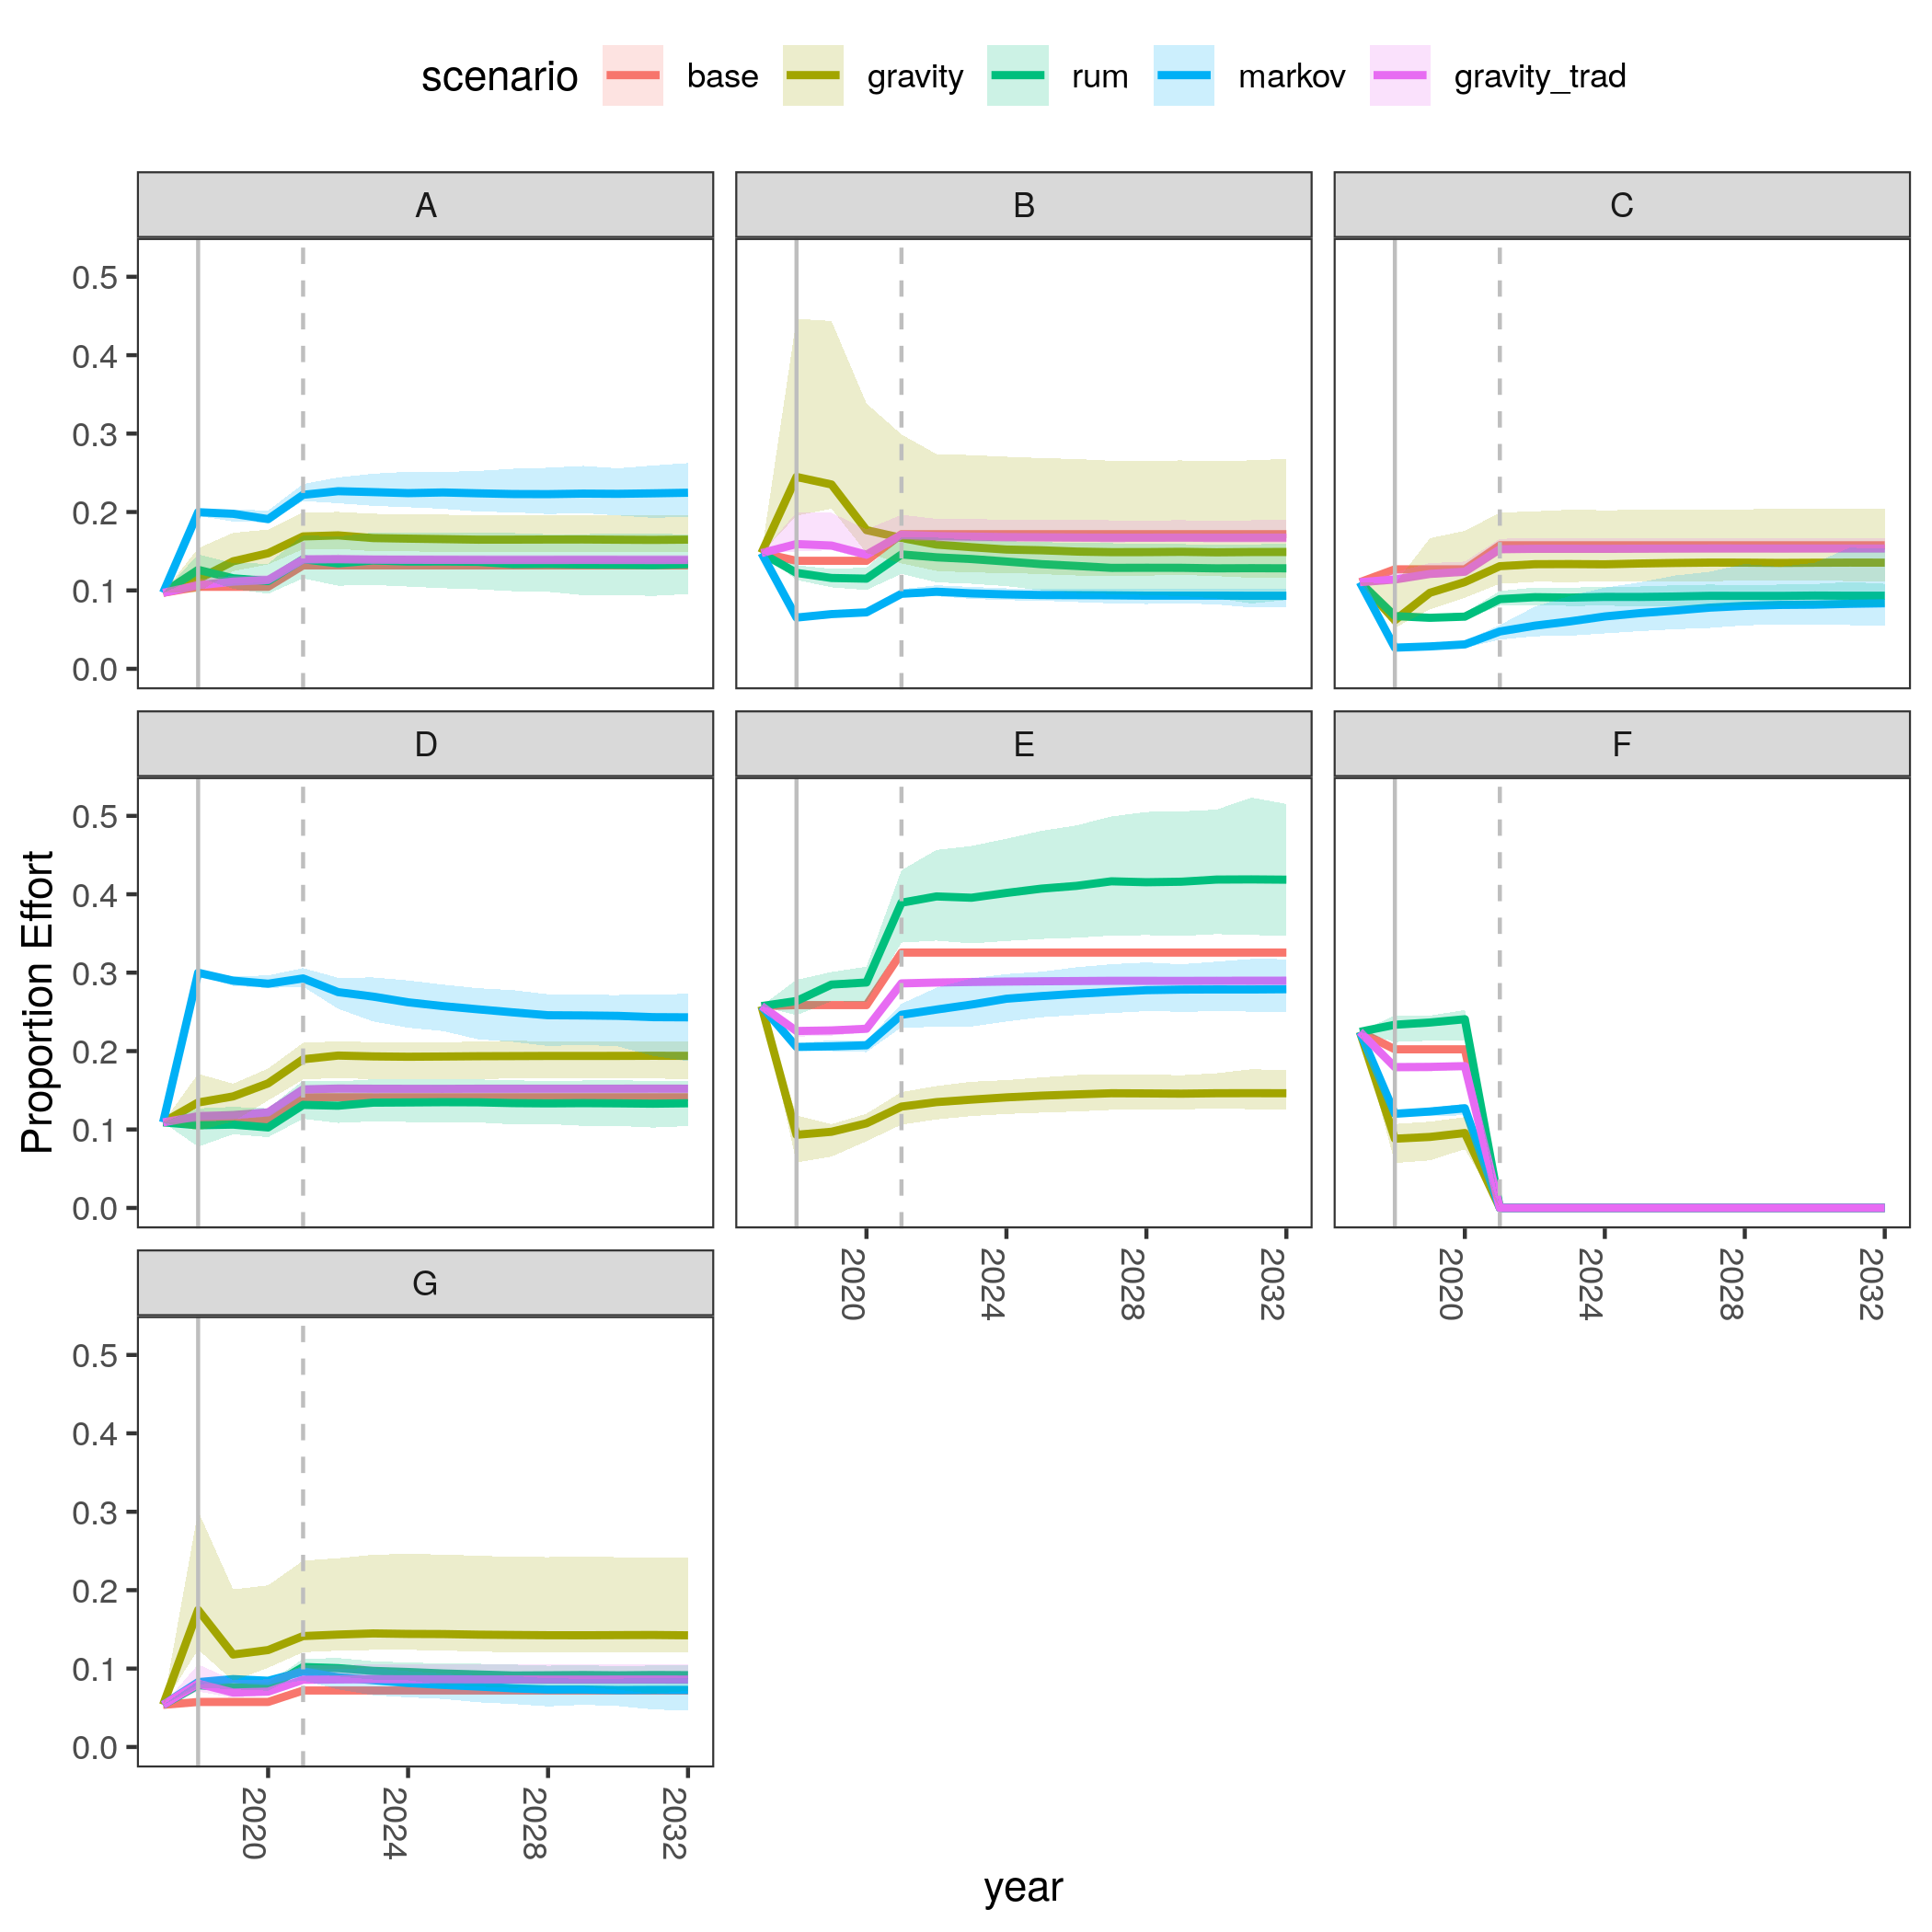
\includegraphics[width=1\linewidth]{figures/Effort_shares_annual}
	\caption{Annual effort share} 
	\label{fig:effort_an}
\end{figure}	

\begin{figure}[!ht]
	\centering
	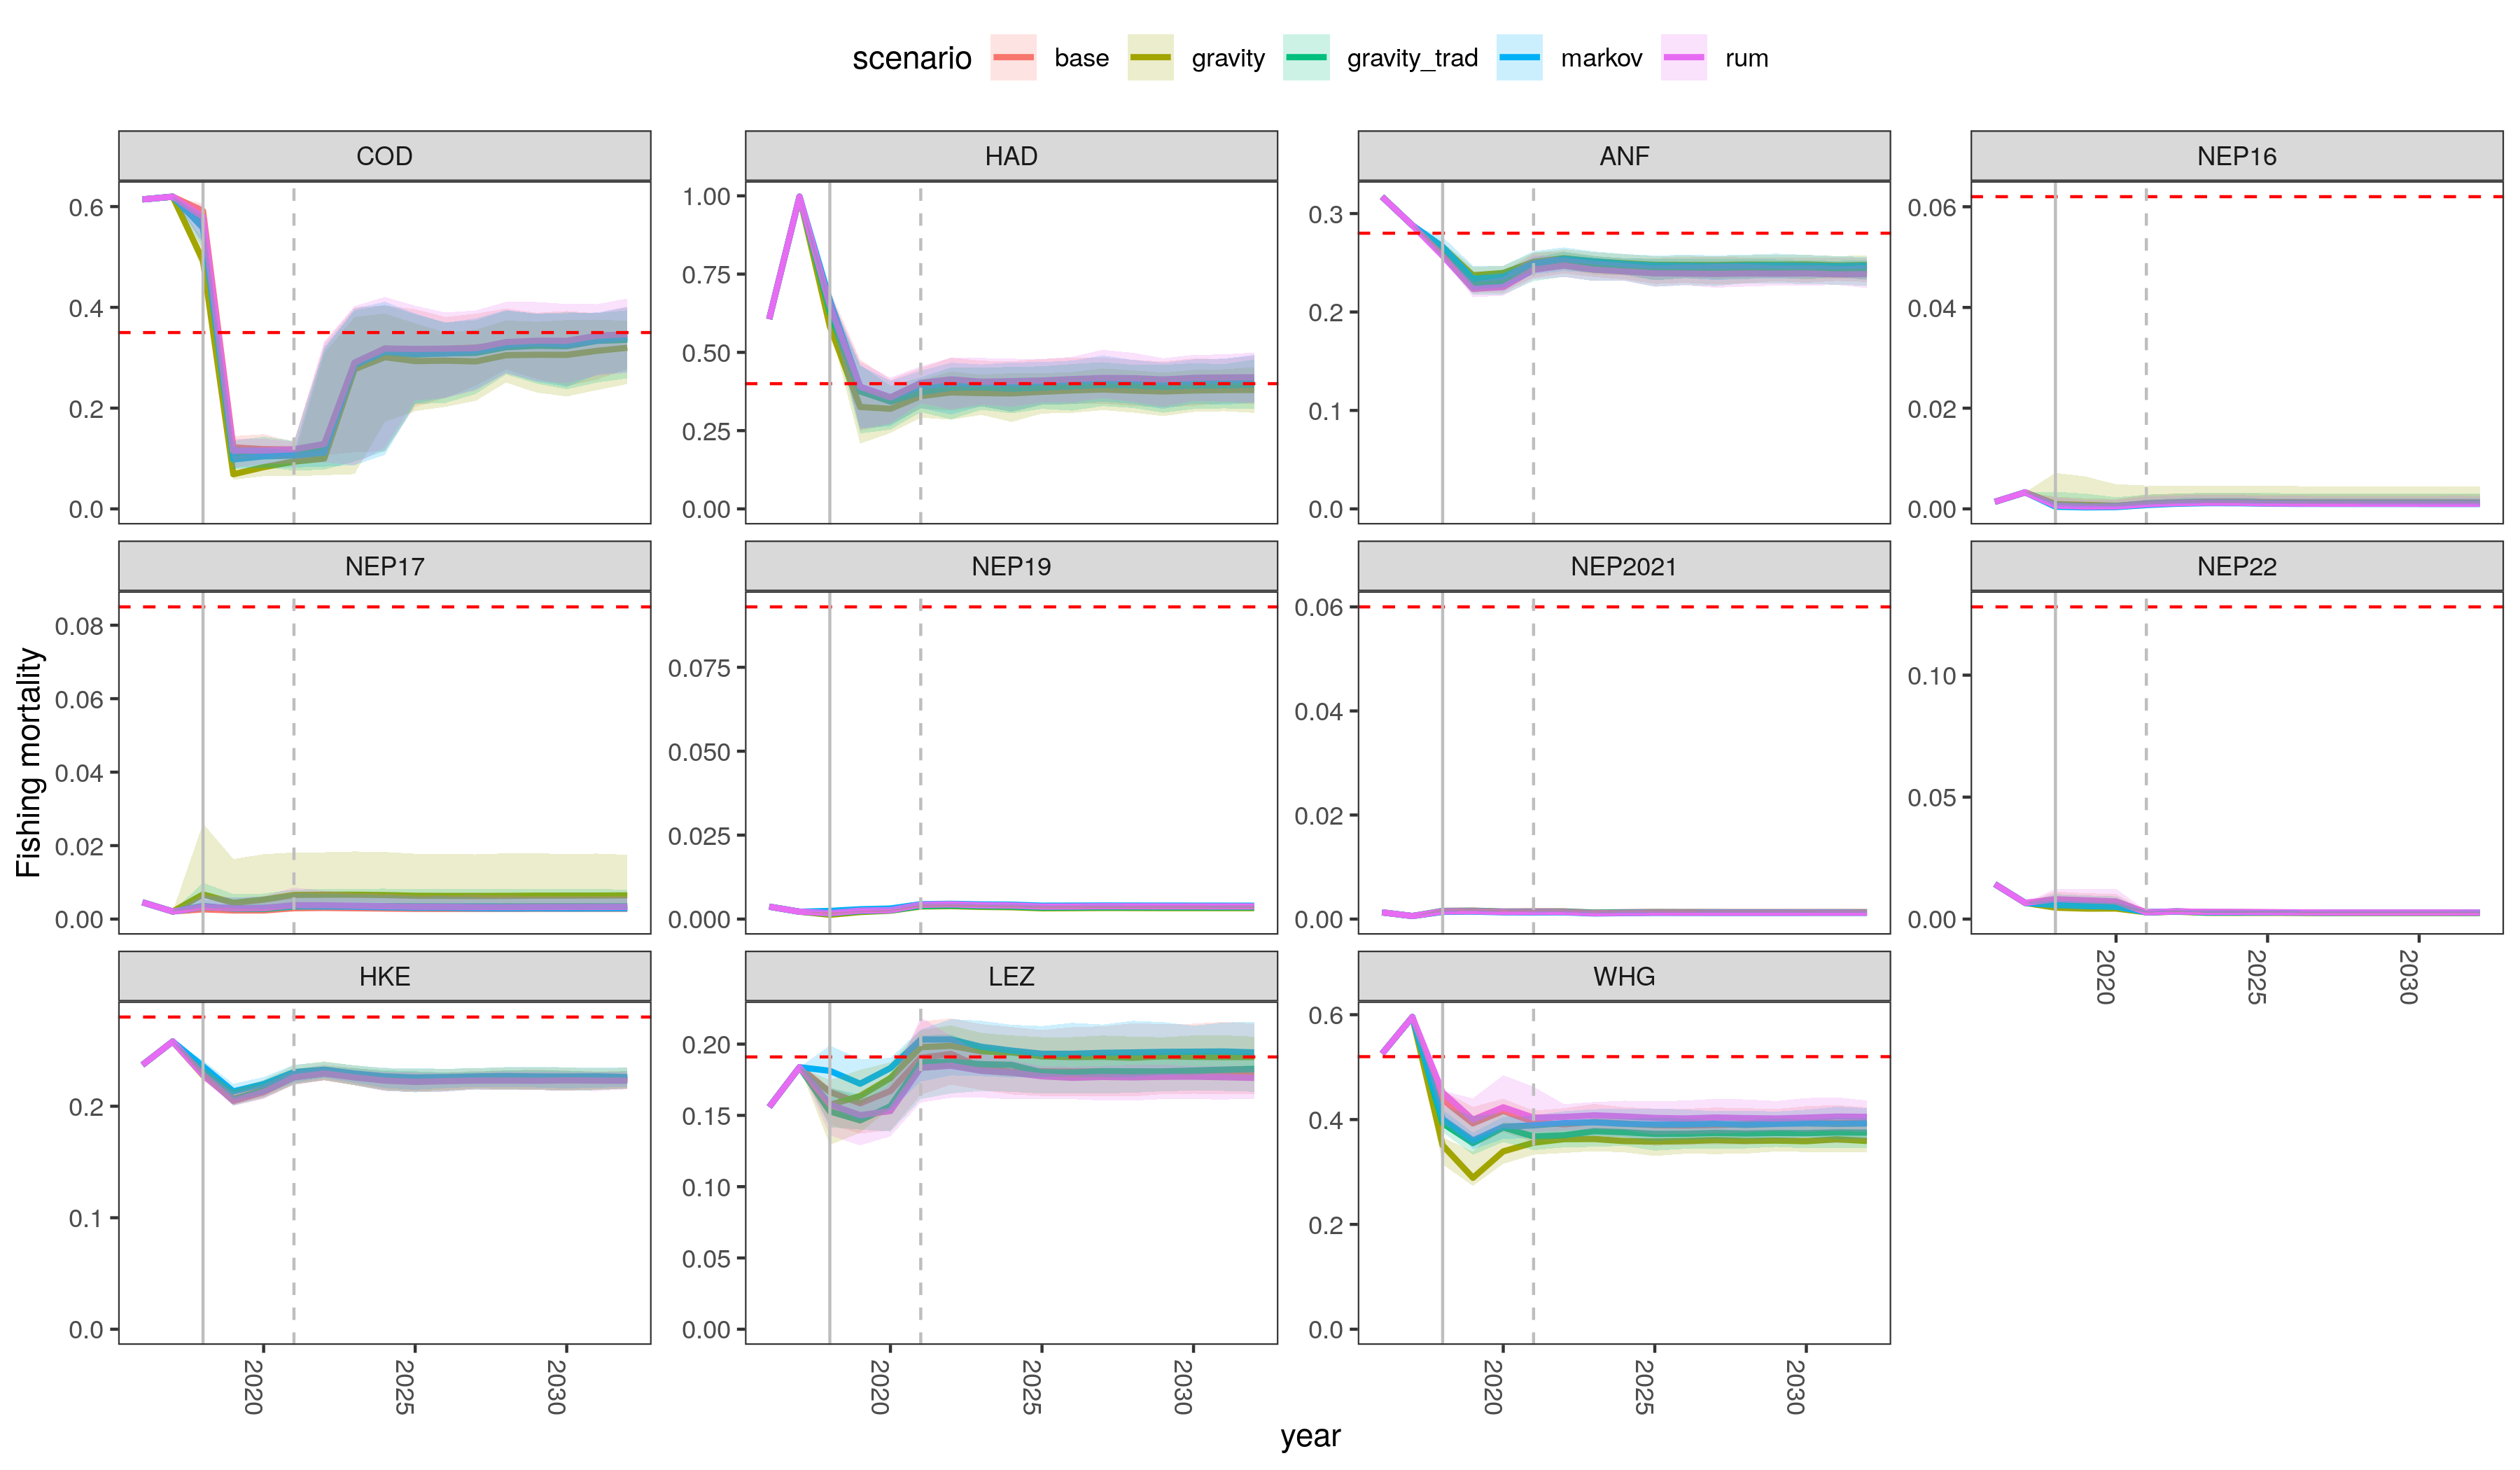
\includegraphics[width=1\linewidth]{figures/F_difference}
	\caption{Fishing mortality per scenario} 
	\label{fig:F}
\end{figure}	

\begin{figure}[!ht]
	\centering
	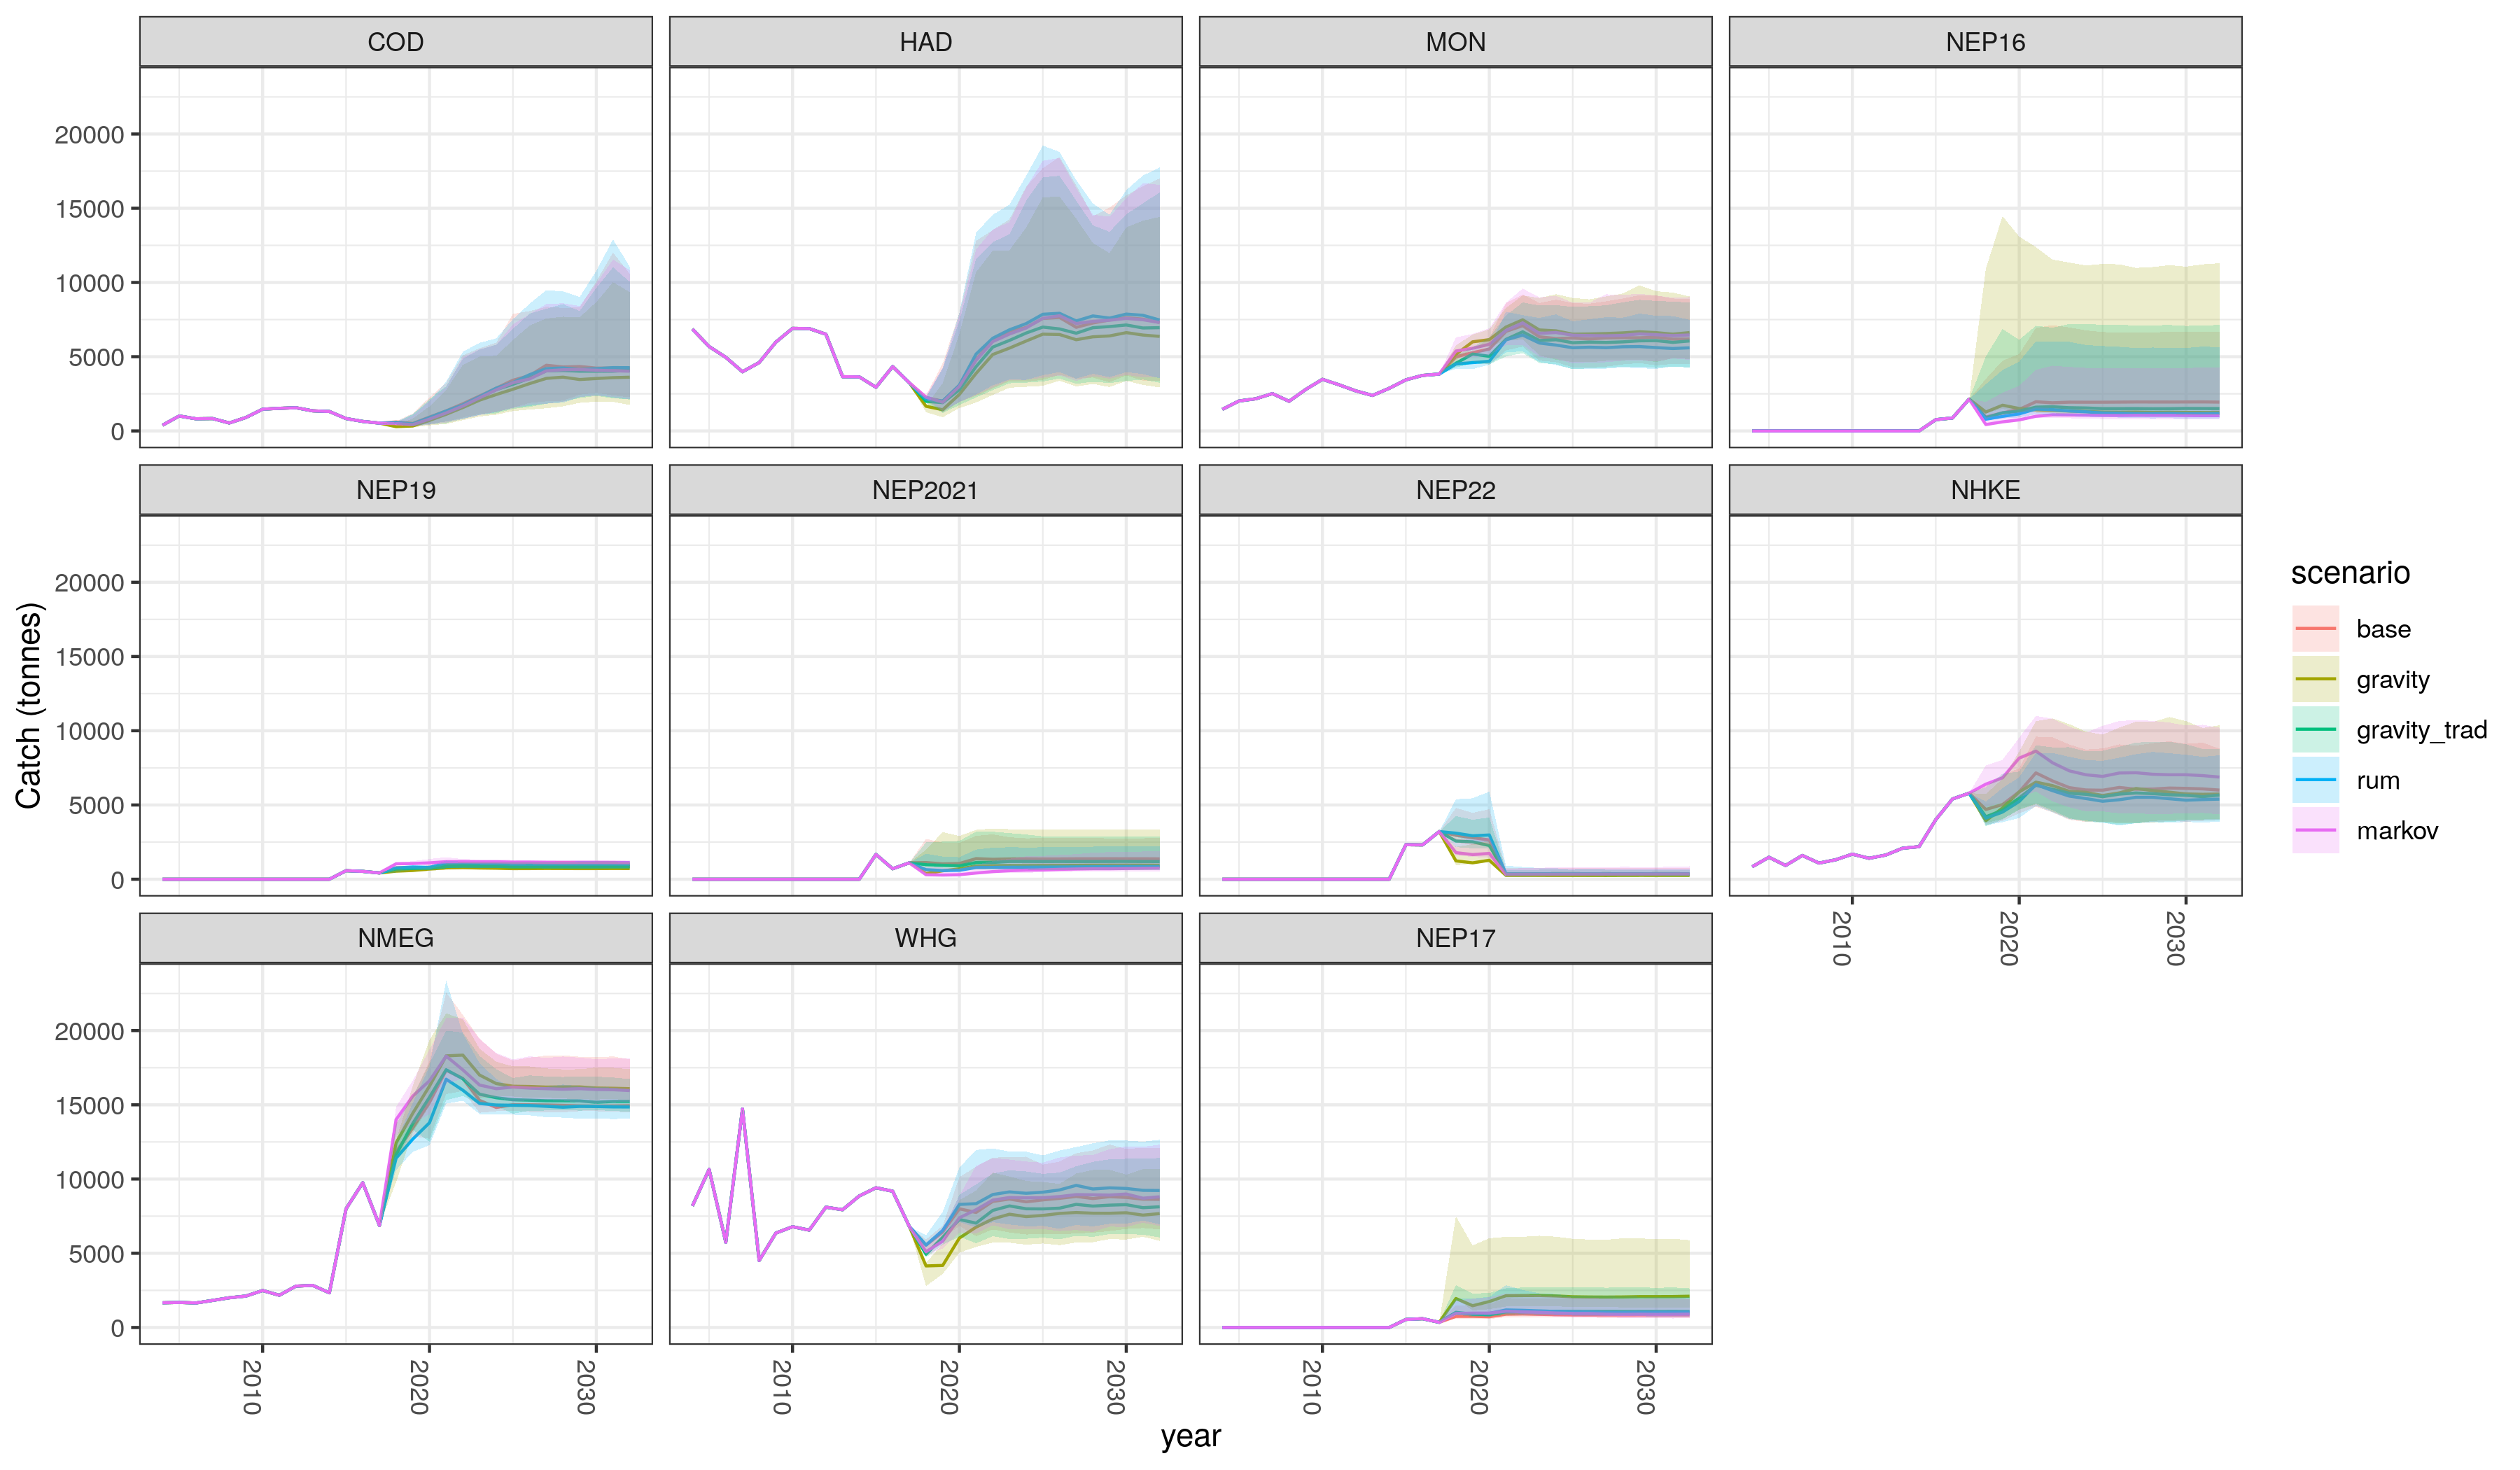
\includegraphics[width=1\linewidth]{figures/IE_Otter_catches}
	\caption{Catches for each stock by Irish Otter trawlers under each
		location model scenario} 
	\label{fig:OtterC}
\end{figure}	

\begin{figure}[!ht]
	\centering
	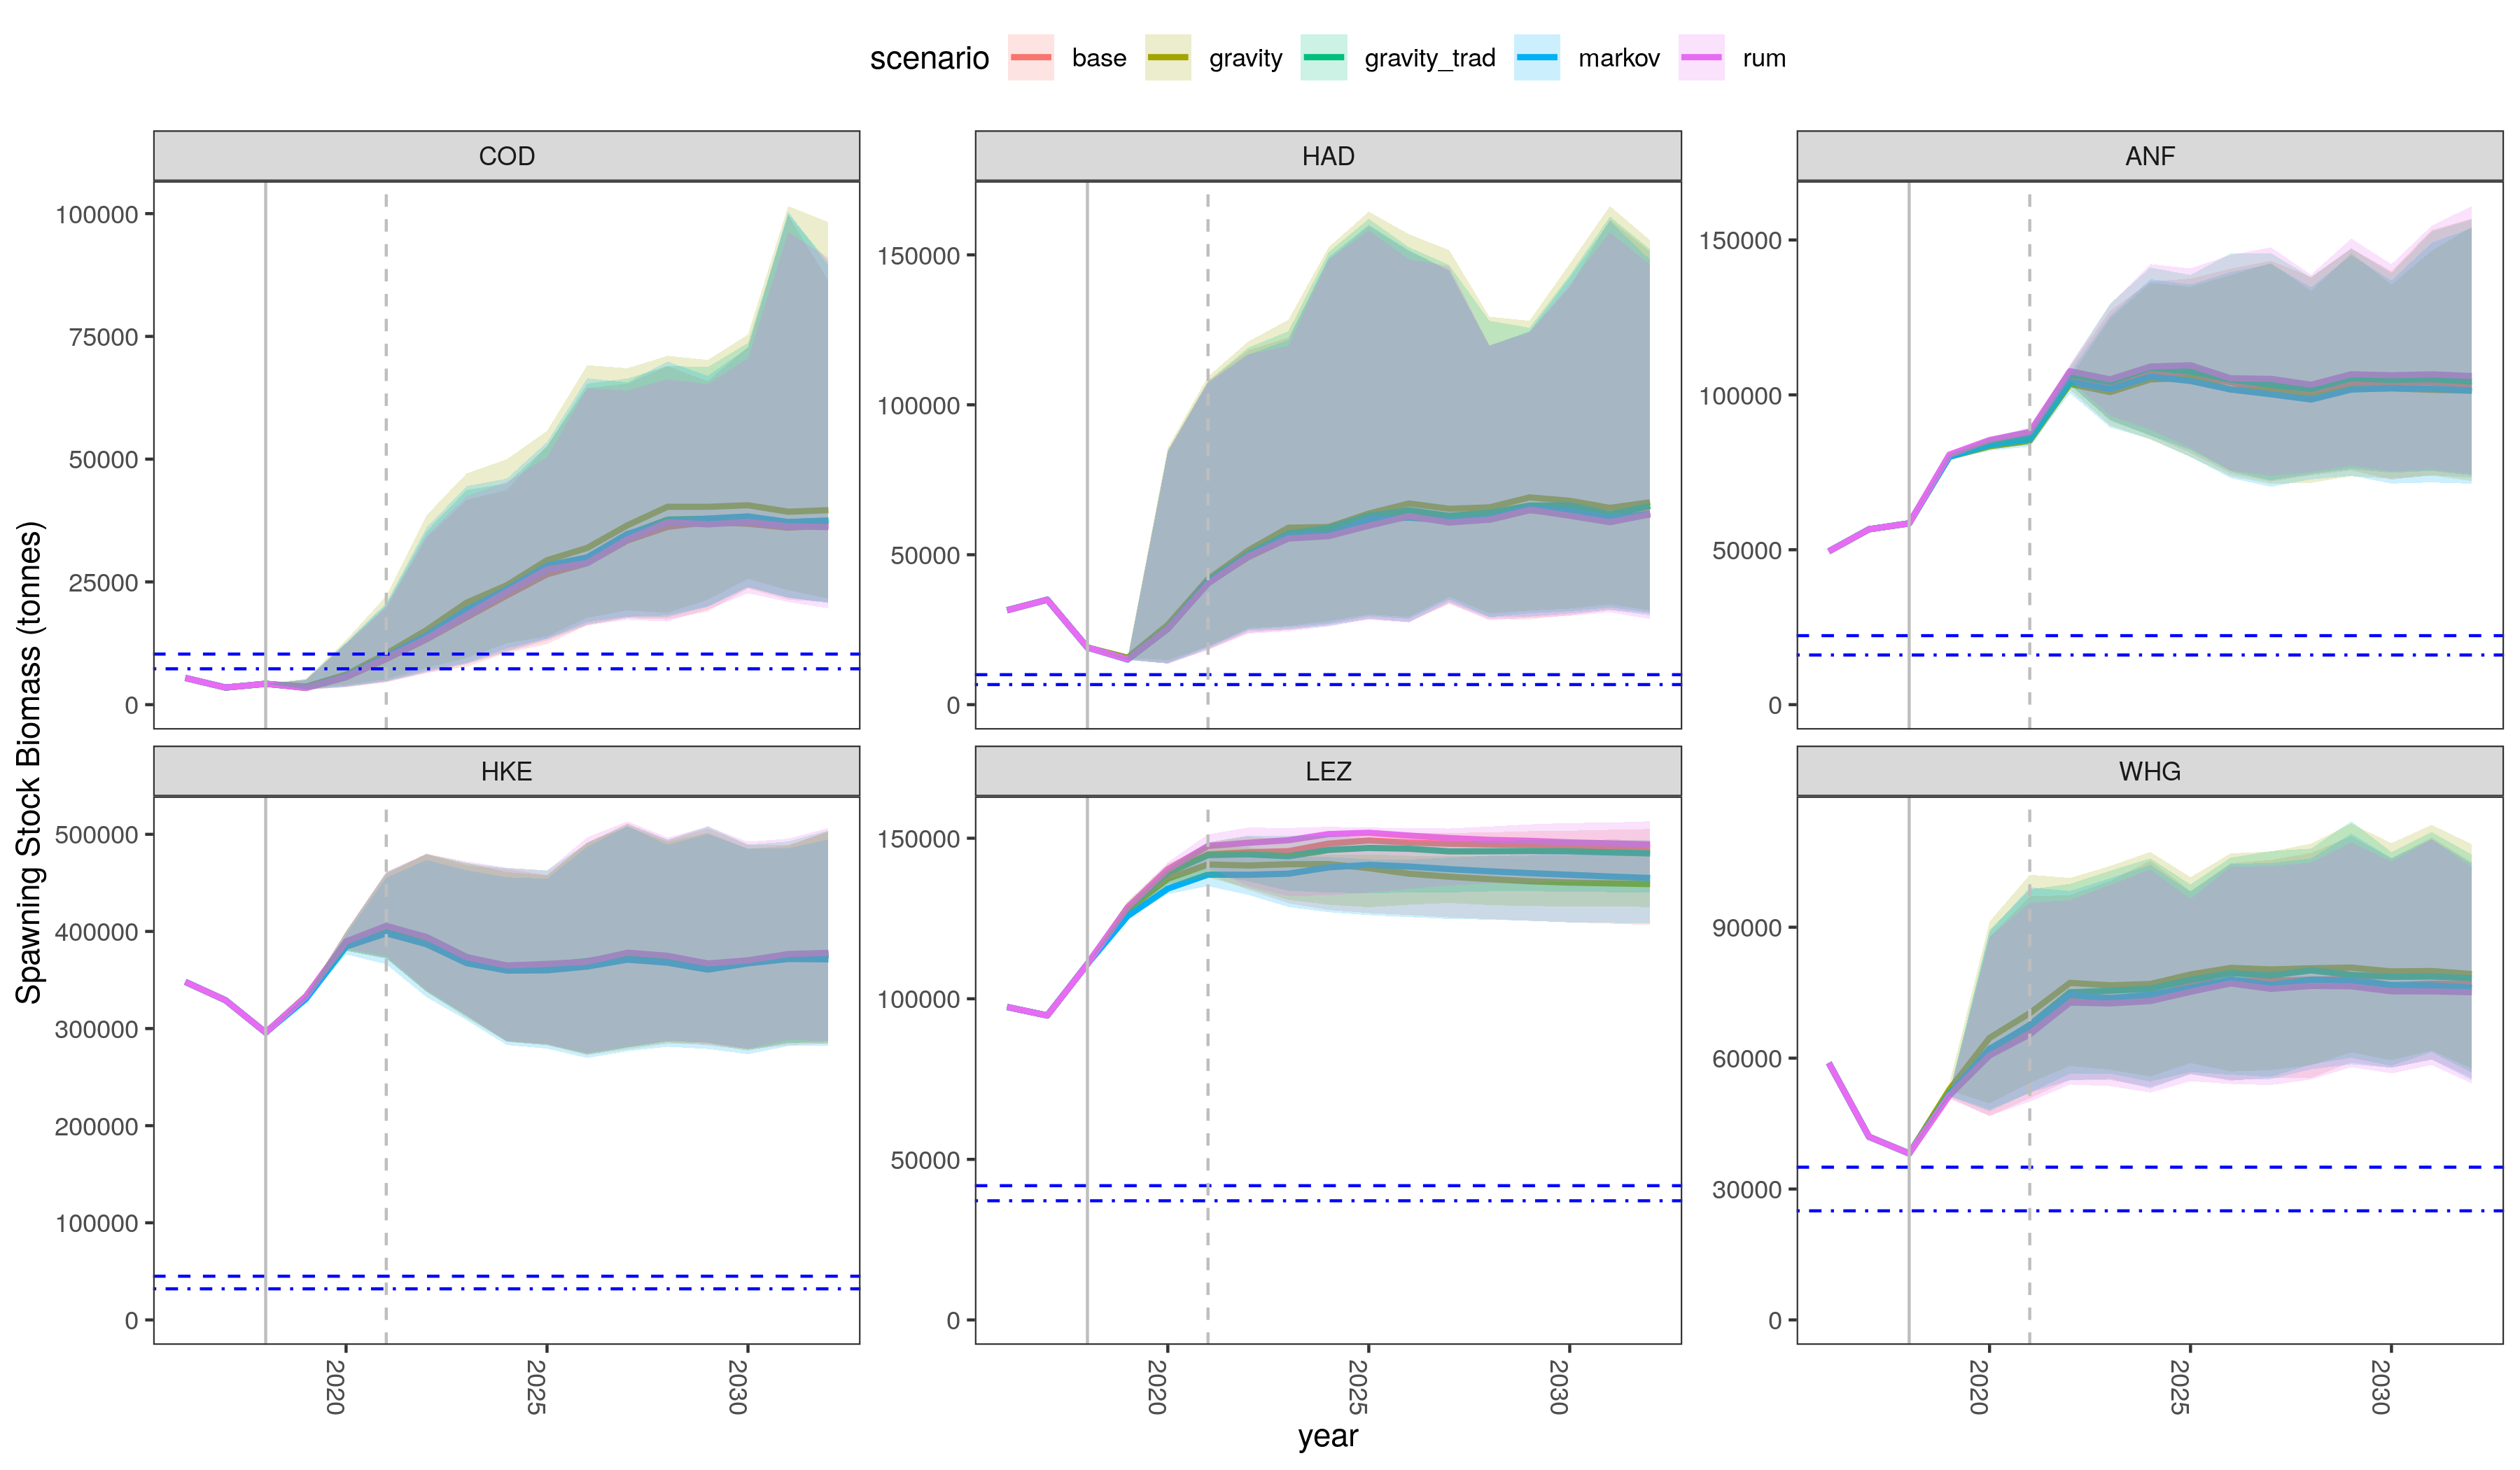
\includegraphics[width=1\linewidth]{figures/SSB_difference}
	\caption{SSB for each stock under each
		location model scenario} 
	\label{fig:SSB}
\end{figure}	

\begin{figure}[!ht]
	\centering
	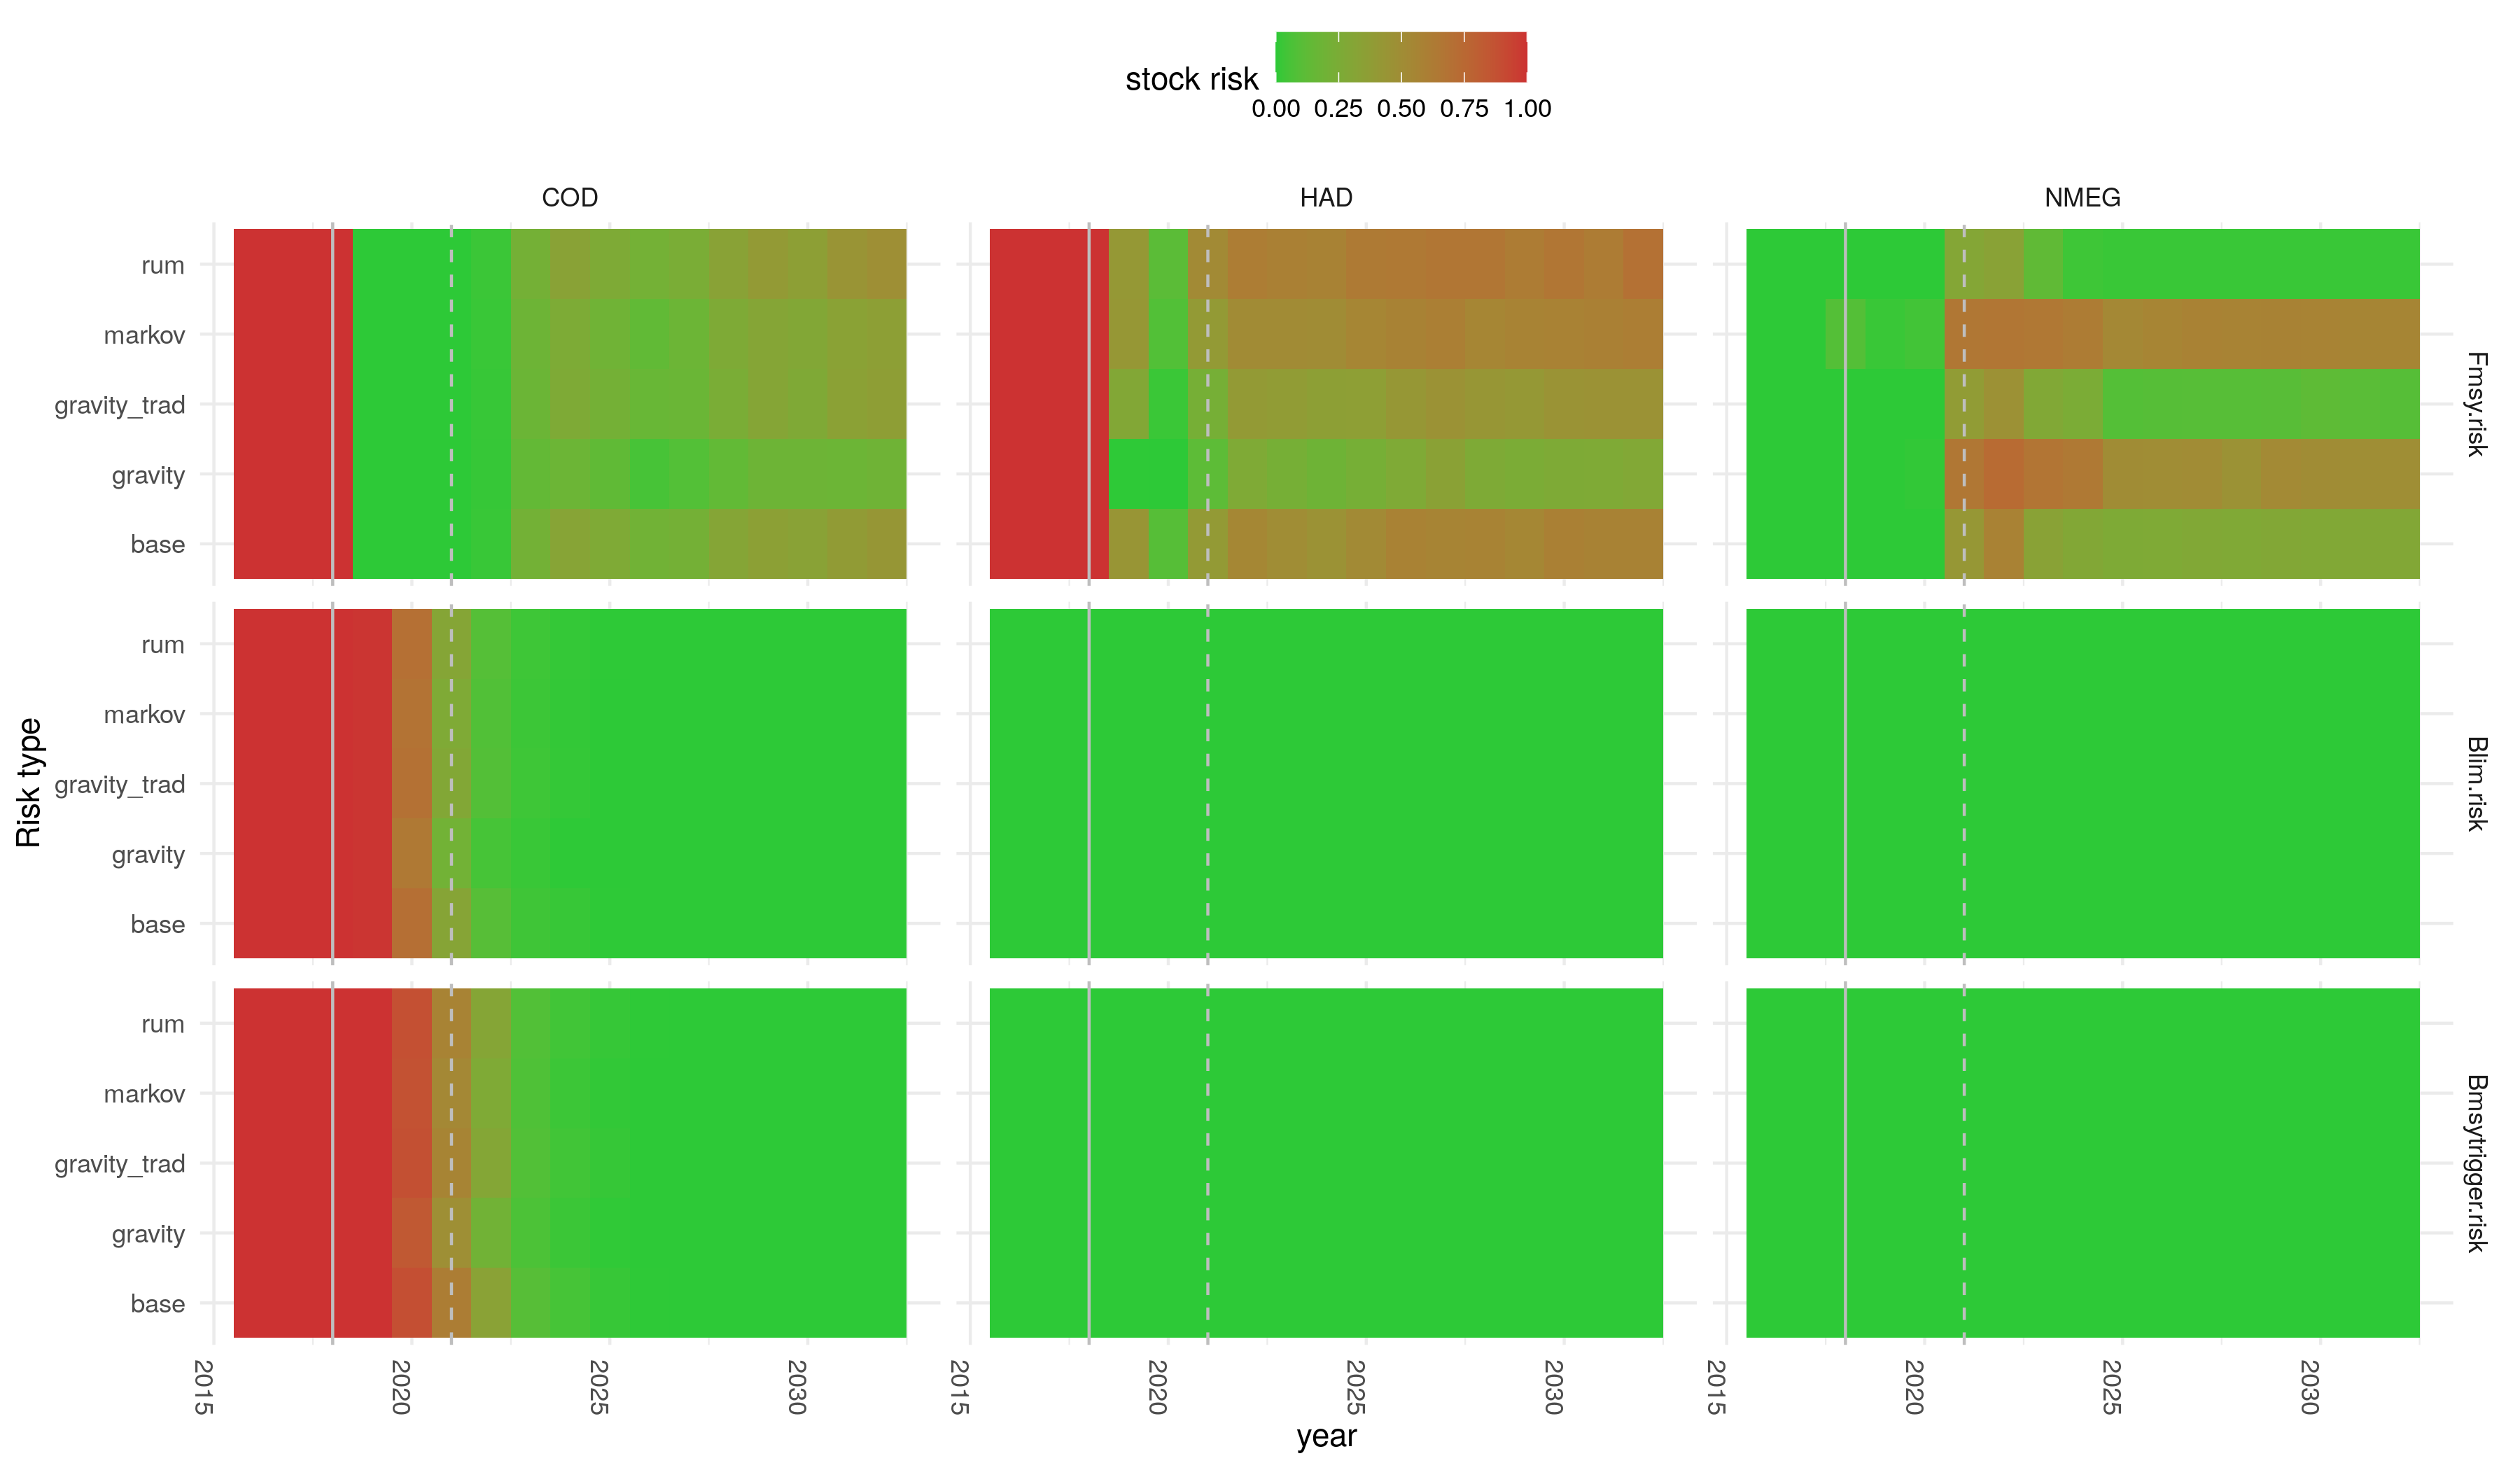
\includegraphics[width=1\linewidth]{figures/stock_risks}
	\caption{Stock indicators per scenario} 
	\label{fig:risk}
\end{figure}	







%%%%%%%%%%%%%%%%%%%%%%%%%
\end{document}
